
\chapter{Presentation, Act 1: Graphs that Make Arguments}

\section{Setting the stage}
Often both learning from a model and making an argument with a model require you to think carefully about how to present data -- to yourself, to your teammate, or to your audience.  The classic example of this is the Morton-Thiokol O-ring failure that led to the destruction of the Space Shuttle Challenger (this was before you were born, so look it up on {\tt wikipedia} if you don't know what I am talking about).  On one hand, at least some of the engineers involved knew that the o-ring design on the booster rocket field joints was much more likely to fail at low temperatures.     But despite their attempts to convince NASA not to launch, NASA leadership made the decision to proceed -- and the shuttle and the astronauts' lives were lost as a consequence.  

While there are any number of ways to dissect this situation, there seems to be little doubt that the way Morton Thiokol made the argument  was a part of the problem.  Edward Tufte's book, {\it Visual Explanations}, provides the graphic that the engineers used to communicate the situation.


\begin{figure}[h!]
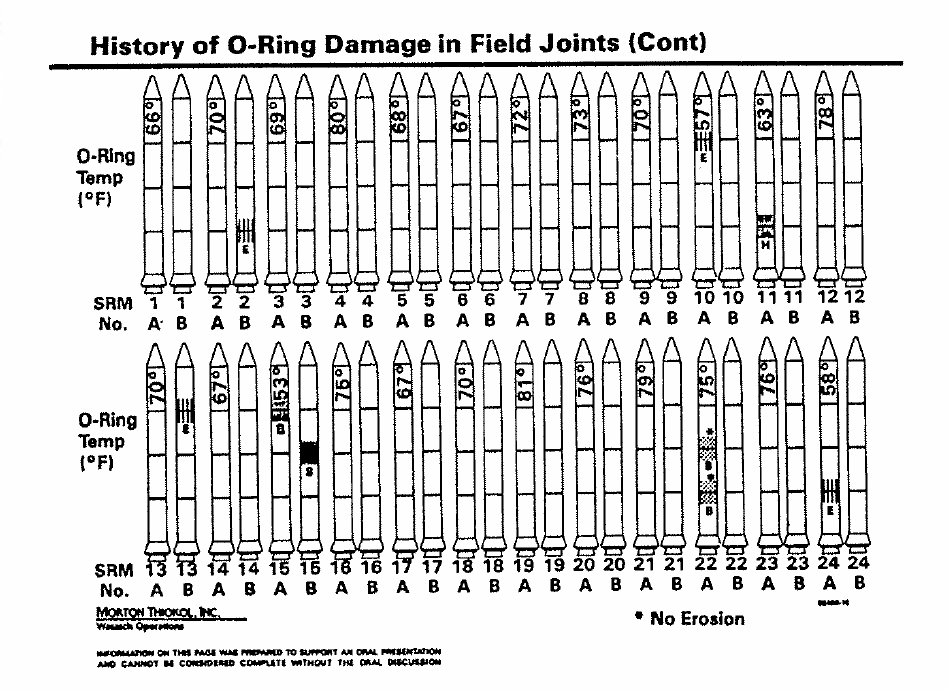
\includegraphics[width=4.5in]{figs/Thiokol1}
\caption{Slide used by Morton-Thiokol engineers to present O-ring damage on 24 previous flights.  Excerpted from Tufte's {\it Visual Explanations}.}
\end{figure}

The graphic shows damage information about 24 previous shuttle flights; the type of damage, location of damage, and outside temperature at the time of the flight are indicated in each pair of booster rockets.  Now, based on this presentation of the information, it is virtually impossible to see if there is any kind of trend here:  not only is there not a legend to indicate what the different damage symbols mean, it also appears that most flights are damage free, and that the damage is randomly distributed.

Tufts suggests an alternative presentation  of the same dataset; he plots the amount of O-ring damage as a function of launch temperature:

\begin{figure*}[h!]
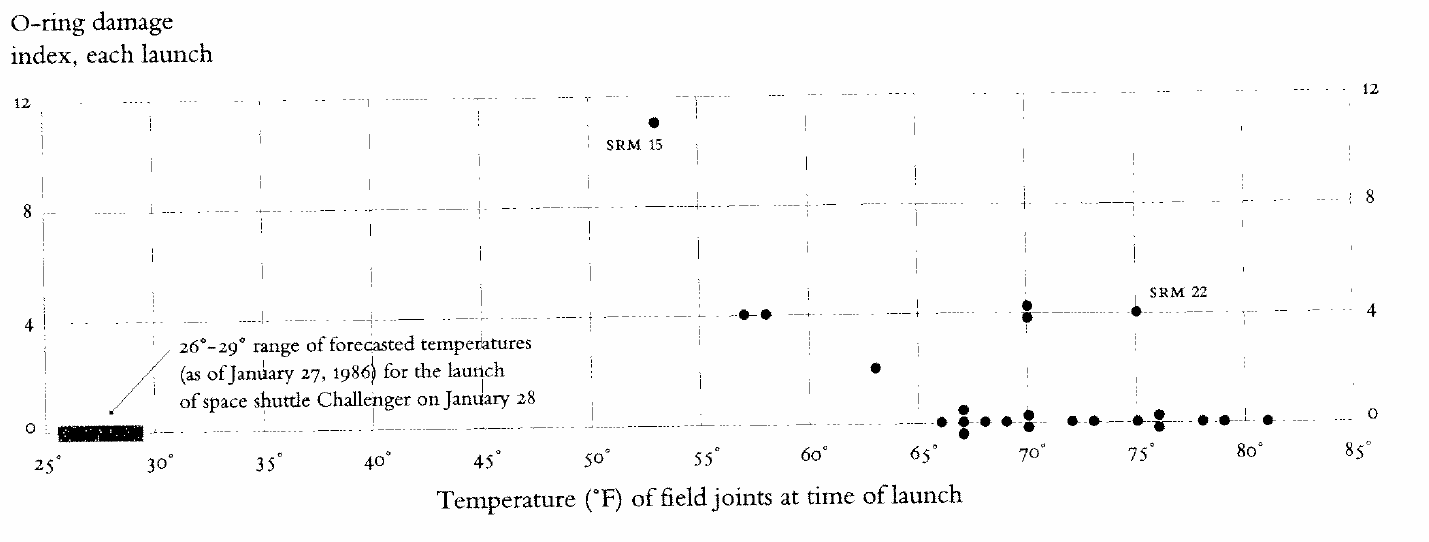
\includegraphics[width=7in]{figs/Thiokol2}
\caption{Tufte's presentation of O-ring damage on 24 previous flights.  Damage index is plotted as a function of temperature; the plot also shows the forecast temperature for the proposed launch date.  Excerpted from Tufte's {\it Visual Explanations}.}
\end{figure*}

If you look at this figure, it seems clear that launching at below 30\textdegree F is probably a bad idea: there seems to be a clear correlation between lower temperature and increased O-ring damage.  The graph makes an {\it argument} -- something that is missing entirely from the first figure.

In this chapter we'll discuss guidelines that should help you to create graphs (and ultimately posters) that help you to make an argument.  Some of these guidelines relate to the graphs and other representations you create as a part of your modeling process.  When you're {\it doing} modeling, making the right graph is often the thing that helps you make good decisions about what directions to pursue, and that helps you identify flaws in your reasoning, in your model, or in your simulation.  We'll also address the question of how to create representations you use in presenting results -- showing someone the work that your model does.  In presentation, the right graph can communicate your point succinctly and convincingly in a way that no amount of text can.

\section{Using Graphs in the Modeling Process}

\subsection{If in doubt, make a plot - or two!}

One of the wonderful things about doing modeling and {\it simulation} is that the cost of making a plot is almost zero:  when you are running a simulation, there's really no reason {\it not} to plot your results. 

This may sound obvious, but as you develop facility with using simulation for zero-finding, optimization, etc., there is a temptation to use the simulation to generate an answer, as opposed to an answer that is accompanied by a graph that illustrates the answer.  {\it Resist this temptation.}  Making the plot will allow you to check that your simulation does what it should - that it's consistent with the qualitative behavior you predicted before you even wrote the simulation.  Ultimately such a plot might also be helpful in convincing an audience that the behavior you are presenting is ``real''.  To quote a politician,``trust but verify.'' 

Recall the simulation we ran for the wolf-moose model.  We found that as the moose birthrate dropped, the amplitude of the moose population oscillation decreased, but then showed a sharp discontinuity at a birthrate of around  $\beta = 0.025$ moose per moose per month.  What was going on there (see the discontinuity in amplitude in Figure 3)?  

\begin{figure}[h!]
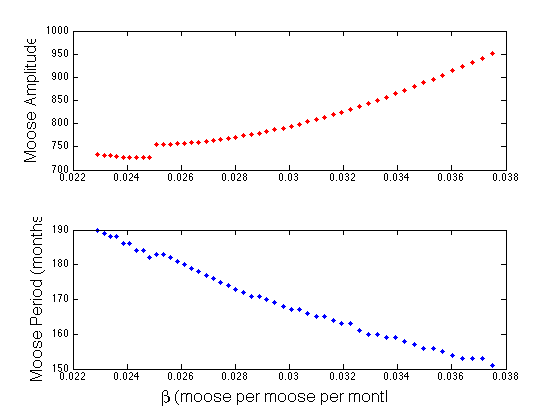
\includegraphics[width=4in]{figs/MooseBCSweep}
\caption{Amplitude and period of moose population for sweep of moose birth rate and critical wolf population $W_c$.  Timestep of one month,  $\gamma = 0.05, M_c = 800, K=1$.}
\end{figure}

An easy way to figure this out is to {\it actually look at the results}.  To do so, I plotted a ``stack'' of the timeseries for the different {\it beta} values.  At a moose birthrate of $\beta = 0.025$ we see a particularly interesting situation:  for this value of $\beta$, the moose population starts at a minimum value.  For larger values of $\beta$, the moose population first increases, goes through a maximum, and then finally reaches its first minimum.  This likely accounts for the discontinuity in amplitude -- if we look back at the approach we used to calculate amplitude, we were measuring the distance between the first zero derivative and the second.  So for $\beta = 0.025$, the {\it location} of this measurement in time suddenly shifts -- yielding a discontinuity in the amplitude. 

It's likely that at this point you're looking at figure 4 and wondering what we're talking about right now.  Indeed, figure 4 probably makes your head hurt a bit -- it takes quite a bit of thought about the problem to make sense of this graph, because it is showing about 40 different time series at once.   

If figure 4 were being used in a presentation, the fact that it makes your head hurt would be a problem.  But it's included here because  it's a figure that {\it I} made to help {\it myself} figure out why a particular effect was taking place (the amplitude discontinuity).  So even though it's not a pretty plot -- and even though it's hard for an audience to interpret -- it's a great graph to have made to support the modeling process.

\begin{figure}[h!]
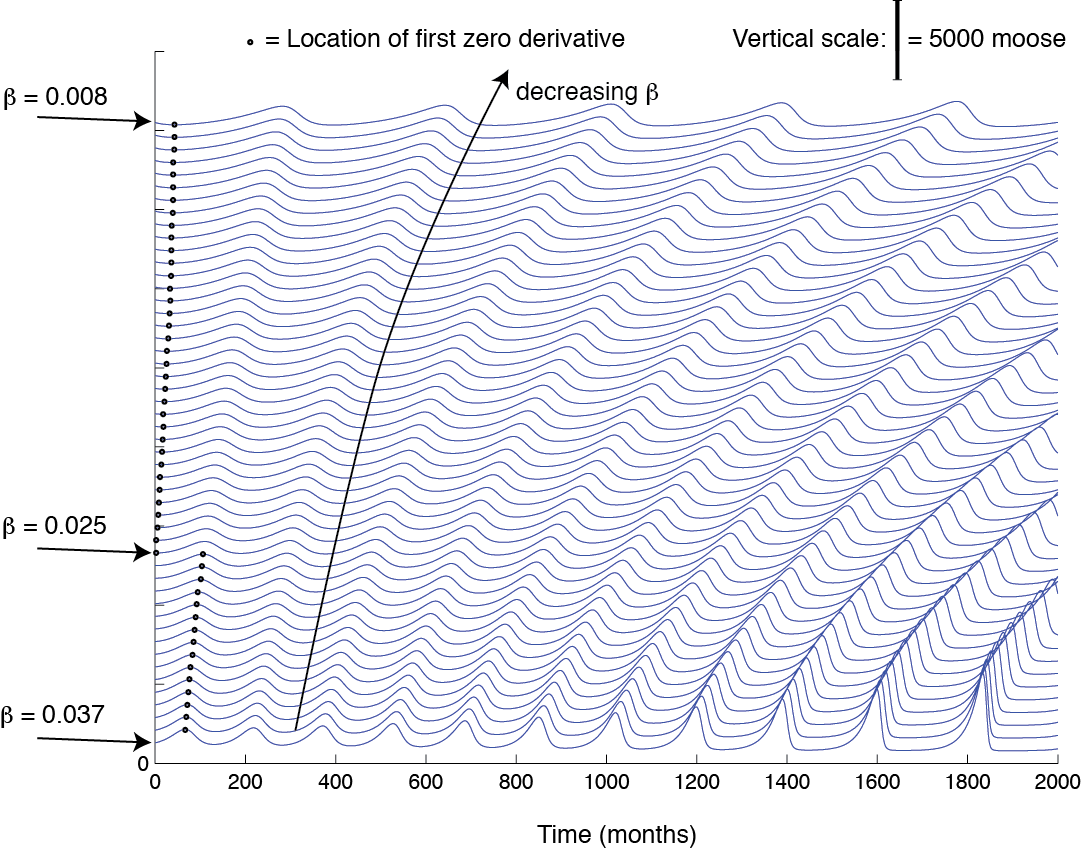
\includegraphics[width=4in]{figs/MooseBCSweepStackWFD}
\caption{Moose time series for different $\beta$ values.  Timestep of one month,  $\gamma = 0.05, M_c = 800, K=1$.  Approximate locations of first zero time derivative in moose population indicated.}
\end{figure}

Figure 4 also indicates that as $\beta$ decreases further, we do get pretty consistent behavior -- so we expect that the increase in amplitude for $\beta < 0.025$ might be ``real'' (not an artifact of our definition), and figure 5 indicates that this is likely the case.
  
\begin{figure}[h!]
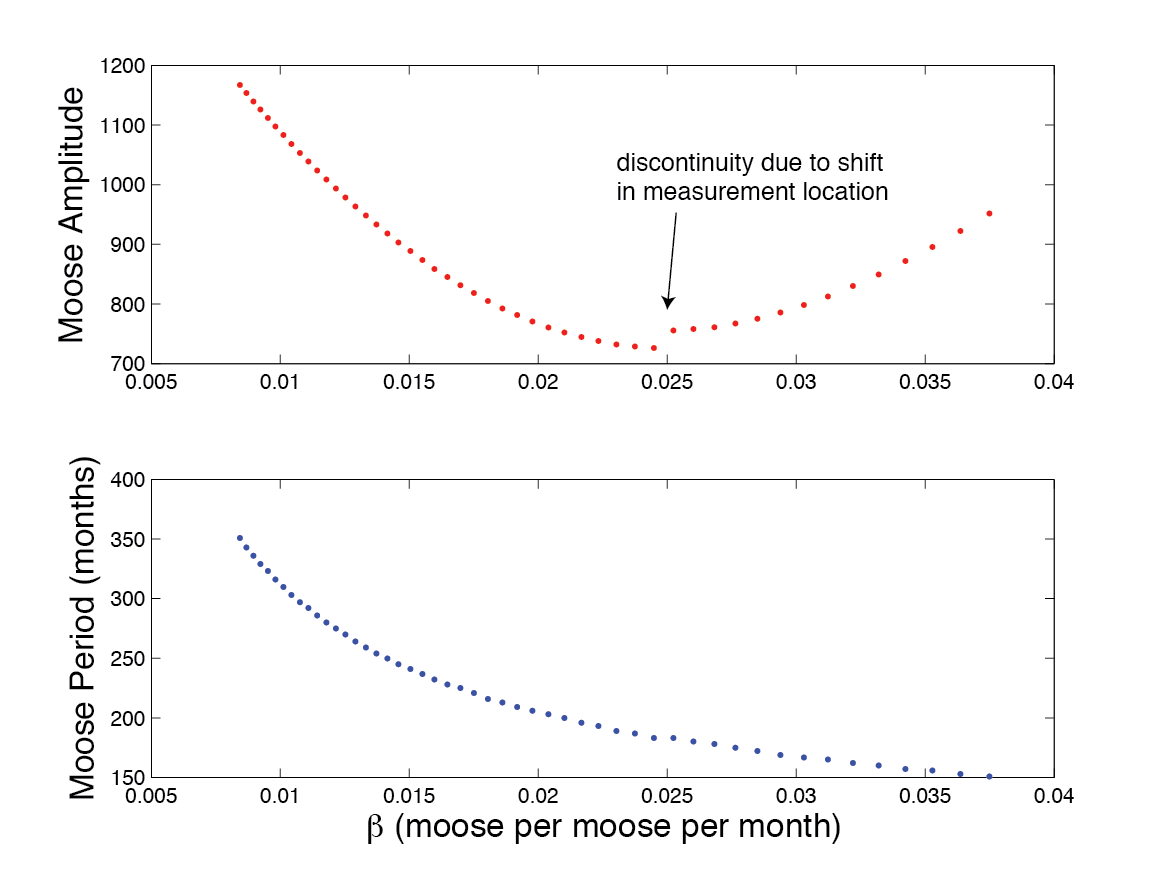
\includegraphics[width=4in]{figs/BroaderBCSweep}
\caption{Amplitude and period of moose population for sweep of moose birth rate and critical wolf population $W_c$.Timestep of one month,  $\gamma = 0.05, M_c = 800, K=1$.}
\end{figure}

\begin{del}
Spend some time making sense of figure 4.  Can you think of a better way of showing why the discontinuity in figures 3 and 5 occurs?
\end{del}
\subsection{Don't be lazy -- digitize!}

A corollary to ``if in doubt, make  a plot''  is ``if in doubt, digitize data from other sources.''   It is common to find yourself relying on a plot from the literature -- think, for example, of the trophic cascade paper in the sharks and scallops project, or of the plot from the Isle Royale website that we looked at in the last chapter.  

In both of these cases, the sources include relatively pretty plots of measured data from the physical system.  When one encounters plots like this, it's awfully tempting to use the plot just as it is -- after all, it is already a ``publication quality'' graph!  Why do the work of measuring the locations of the data points, collecting them all in MATLAB, etc., only to create the plot again?

{\it Resist the temptation} to just reproduce a graph from a paper, and do the additional work of digitizing the data so that you have the actual numbers.  This approach has a number of advantages:

\begin{enumerate}
\item Digitizing allows you to explore the data more efficiently (e.g., ``gee, I wonder what it would look like if I plotted this logarithmically?'');
\item Digitizing allows you to use the data to do calculations of parameters (e.g., ``gee, I wonder how the change in the moose population correlates with the number of wolves?'');
\item Digitizing allows you to make plots of both data and model on one axis, which can be very helpful in making the argument that a model has the right behavior (``gee, look, the data and the model actually line up!''); and
\item From a presentation perspective, digitizing allows you to plot the data in a way that is graphically consistent with the rest of your poster (``Look, all the graphs on this poster actually use the same font!''), 
\end{enumerate}

For example, in the case of Isle Royale, we easily found a figure that showed wolf and moose populations as a function of time.  We could argue that the model and our simulation show about the same behavior by showing this plot, and then showing a plot of the simulation results:

\begin{figure}[h!]
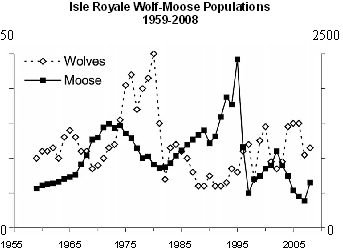
\includegraphics[width=4in]{figs/wolfmoosedata.jpg}
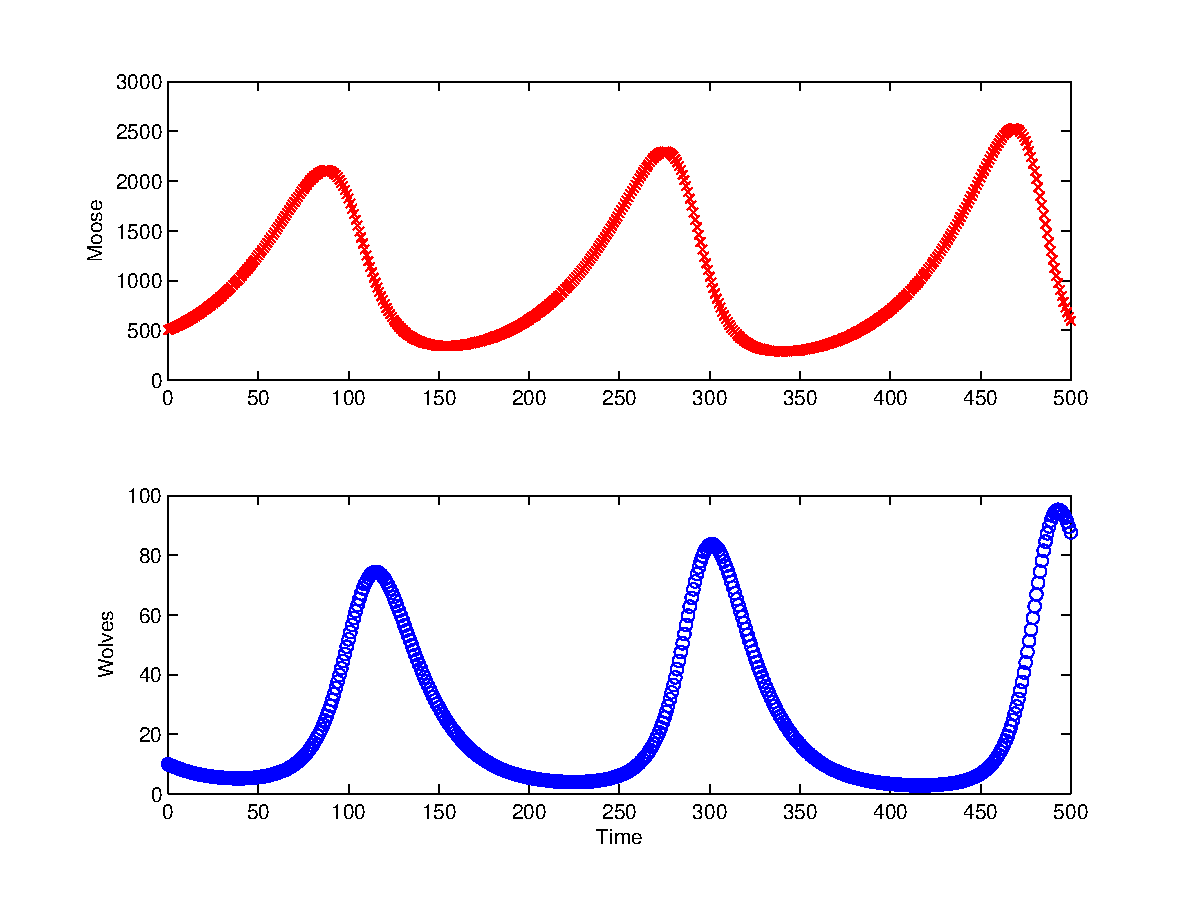
\includegraphics[width=4in]{figs/StackedWolfMooseTimeSeries}
\caption{A really bad and somewhat dishonest comparison of model results and measured data  for Wolf-Moose system. Timestep of one month,   $\beta = 0.025, \gamma = 0.057, W_c = 25, M_c=1000, M(1) = 500, W(1) = 10$}
\end{figure}

Now at first glance, this comparison seems reasonable (or perhaps I should say reasonable-ish).  The wolves and moose oscillate, the peaks kind of seem to match, it's all good -- right?

{\it Wrong.} Let's  look first at the axes.  The simulation has a timestep of months (which we need to look to the caption to learn!), while the plot from the literature is in years.  Furthermore, the length of the axes differ substantially -- so as a consequence, it is nearly impossible to decide whether the data shows similar, substantially longer, or substantially shorter period than the data.  The fact that it {\it looks} similar doesn't mean it actually is.  By the same token, the y-axis scale differs by a factor of two numerically for the wolves (0 to 50 versus 0 to 100), and then by {\it another} factor of two graphically.

We'll also take a look at the presentation of the data.  The {\it data} for moose is plotted as black squares, while the {\it simulation} for moose is plotted with red crosses.  As a consequence, it is very difficult to remember what you are actually looking at -- you can frequently find youself comparing the moose experimental oscillation with the wolf simulation oscillation, due to this inconsistency.

These problems largely disappear if you plot both the simulation and the data on the same axes.  This allows you to see the extent to which they match both qualitatively and quantitatively; it also allows you to adjust parameters easily, should you decide that you need to do so. 

\begin{figure}[h!]
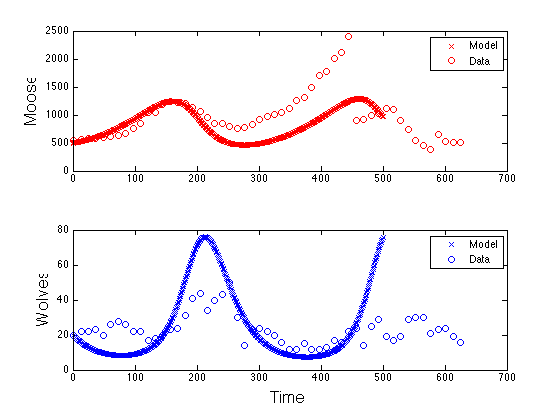
\includegraphics[width=4in]{figs/ModelDataComparison}
\caption{Comparison of model results and measured data  for Wolf-Moose system. Timestep of one month,  $\beta = 0.01, \gamma = 0.05, W_c = 30, M_c=800, M(1) = 500, W(1) = 20$.}
\end{figure}


\subsection{Facilitate comparison}

Digitizing your data is one part of a more general rule:  {\it you should always make choices in plotting that allow you to compare the things you are interested in}.  Of course, in the case of comparing data and model, having both on the same plot allows that comparison in a much more meaningful way than having them in two separate plots.  

But let's think about some examples that only involve model results.  For example, in the Isle Royale case, the simulation produces a timeseries for wolf populations and a timeseries for moose population.  What might you want to {\em compare} for these two timeseries?  

One thing you might be interested in is the way in which the two populations vary relative to each other:  when moose populations peak, relative to when wolf population peak.  You might also be interested in the {\it relative} abundance of wolves or moose.  And of course, you might be interested in knowing the absolute values of the populations:  how many moose, and how many wolves exist at a given time.

If you didn't think about what you want to compare in advance, you might end up making some relatively useless plots.  One bad option would be to plot these two series include using the same y axis for both, in which case you can't really compare the behavior of the wolves to the behavior of the moose because {\it you can't see the wolf behavior}.   This plot does allow you to see something about when populations peak, but besides that it's hard to say anything about the wolf populations.

\begin{figure}[h!]
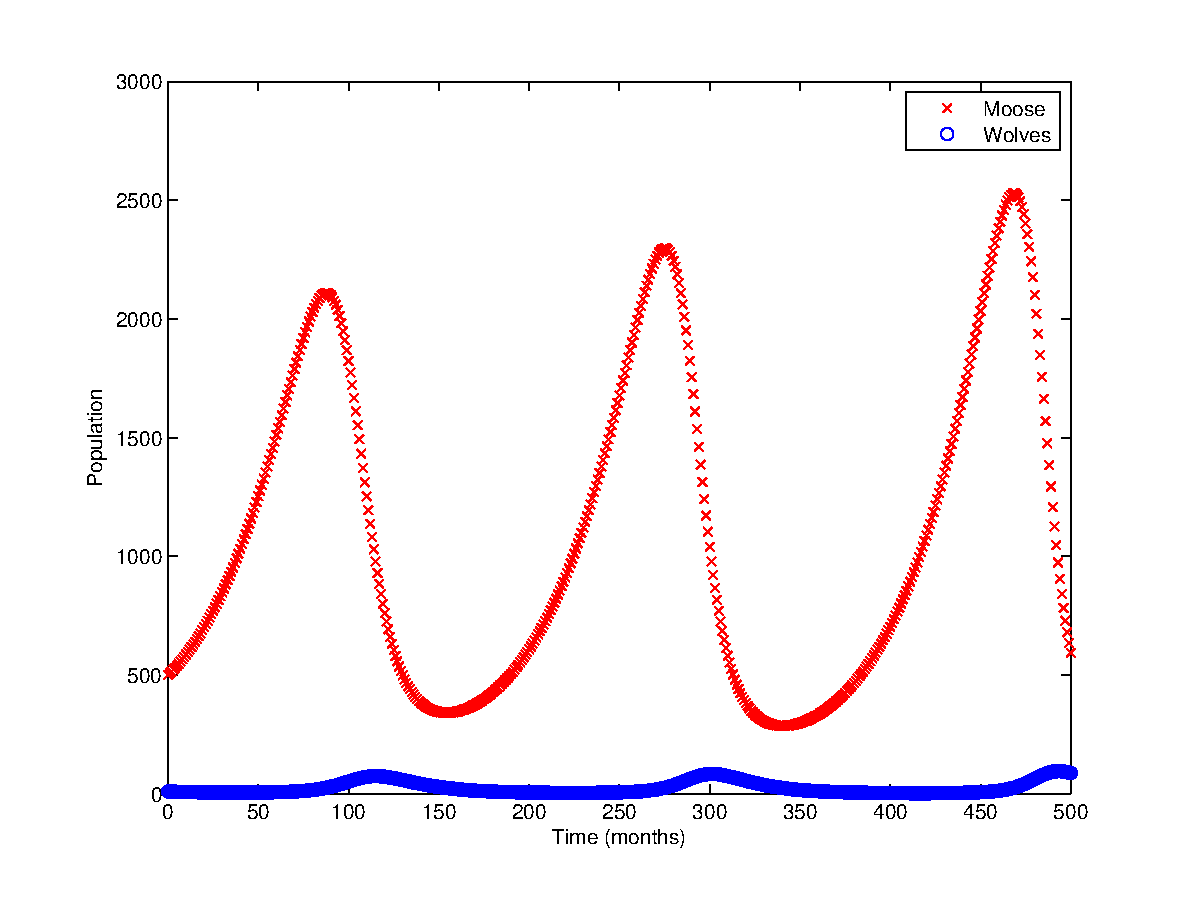
\includegraphics[width=4in]{figs/WolfMooseTimeSeries}
\caption{Simple Lotka-Volterra timeseries results for Wolf-Moose system with a timestep of one month.  $\beta = 0.025, \gamma = 0.057, W_c = 25, M_c=1000, M(1) = 500, W(1) = 10$.}
\end{figure}

A second bad option would be to plot the two populations side-by-side.  This allows us to see what the moose do, and to see what the wolves do, but it makes it very hard indeed to compare the relative behavior of two populations - you keep having to shift back and forth between two time axes.

\begin{figure}[h!]
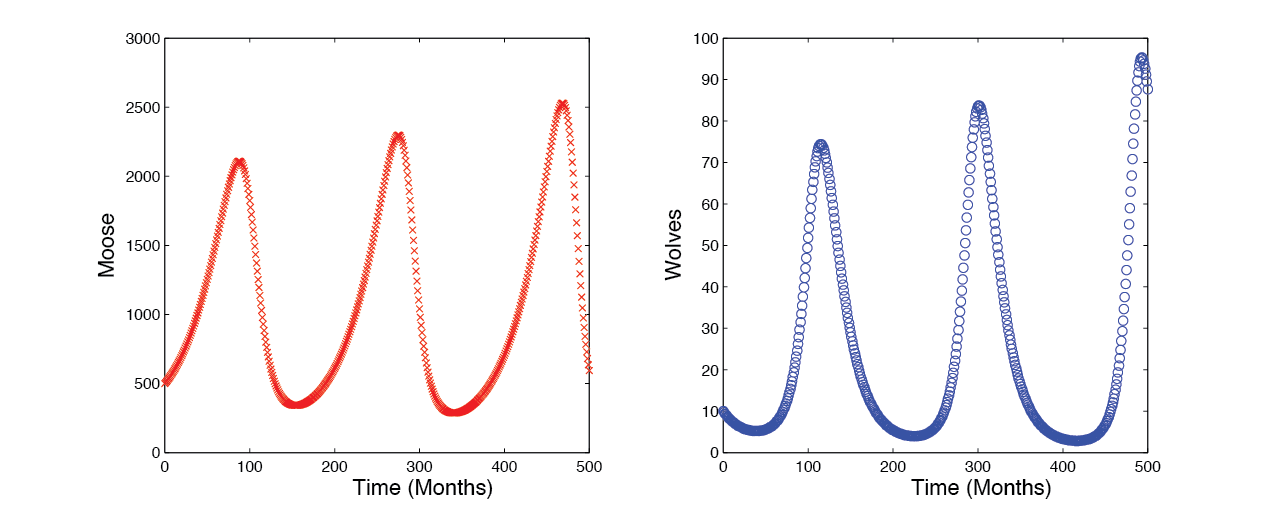
\includegraphics[width=4in]{figs/WolfMooseTimeSeriesHorizontal}
\caption{Horizontal comparison of Lotka-Volterra timeseries results for Wolf-Moose system with a timestep of one month.  $\beta = 0.025, \gamma = 0.057, W_c = 25, M_c=1000, M(1) = 500, W(1) = 10$.}
\end{figure}

Better options include the stacked plots we used in the last section.  This approach gives us one effective time axis, which facilitates the comparison in time of the two populations.  And of course, the most effective approach would be to do the same thing that the data plot did:  put them on the SAME time axis, with two different y axes.  MATLAB will do this quite happily through {\tt plotyy}. See below for examples of both of these approaches.

\begin{figure}
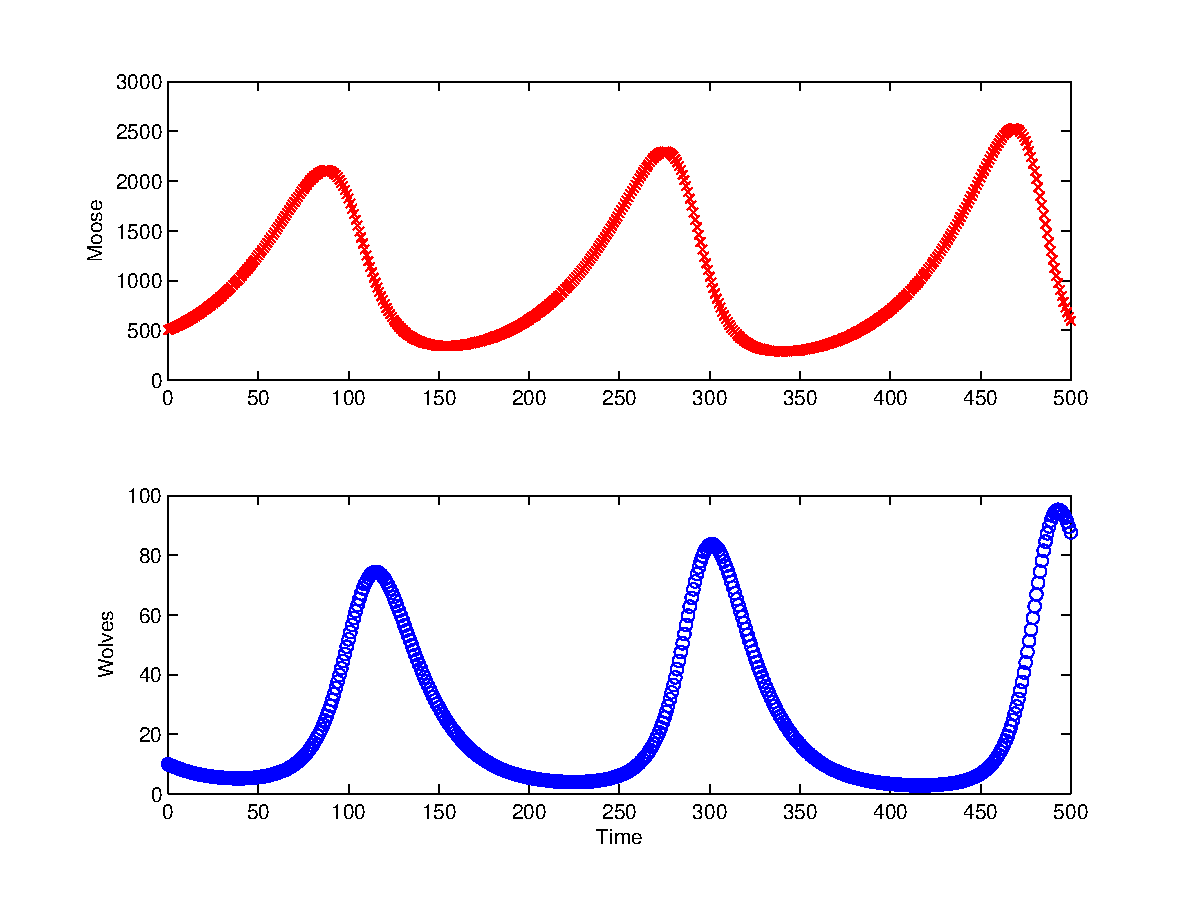
\includegraphics[width=4in]{figs/StackedWolfMooseTimeSeries}
\caption{Stacked (vertical) comparison of timeseries resutls for Wolf-Moose System. Timestep of one month,   $\beta = 0.025, \gamma = 0.057, W_c = 25, M_c=1000, M(1) = 500, W(1) = 10$}
\end{figure}



\begin{figure}
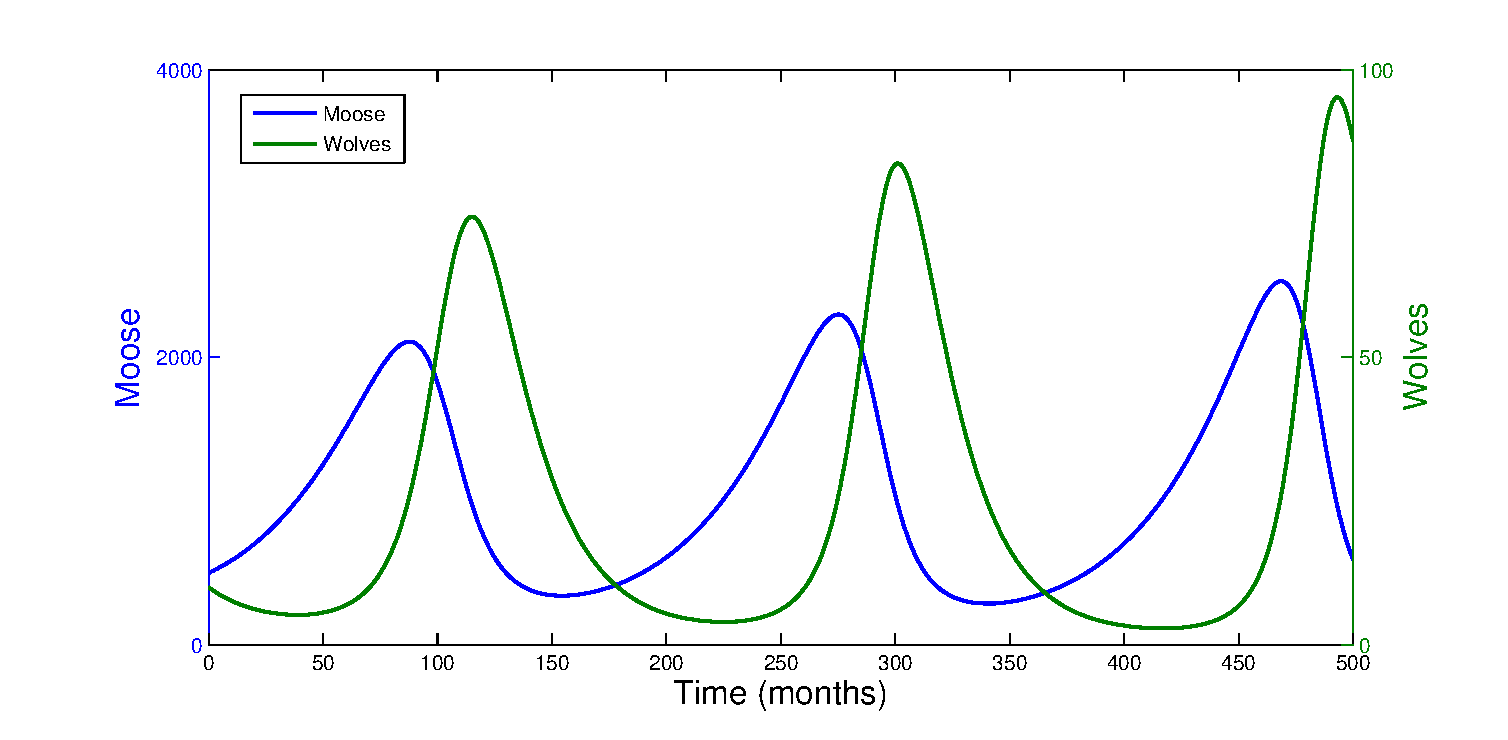
\includegraphics[width=4in]{figs/CombinedWolfMooseTimeSeries}
\caption{Comparison of timeseries results using two y-axes for Wolf-Moose System. Timestep of one month,   $\beta = 0.025, \gamma = 0.057, W_c = 25, M_c=1000, M(1) = 500, W(1) = 10$}
\end{figure}

In general, models tend to produce multiple quantities, and some of those quantities can be much larger than others.  Wolves and moose are a pretty mild example of this; if you think about a model that includes beetle eggs, adult beetles, and trees, it's easy to imagine that each quantity might be multiple orders of magnitude larger or smaller than other quantities. Presumably the number of eggs might be  hundreds of times larger than the number of beetles, which in turn might be hundreds or thousands  of times higher than the number of trees (or, alternatively, the biomass of beetles might be me much lower than the biomass of trees!).  In this kind of situation, another option is to use the power of the logarithm to examine model results that span multiple orders of magnitude.  This of course has the advantage of allowing you to plot everything on one y-axis, and allows you to see behavior in all the quantities you are plotting -- even if you're plotting more than one thing.  To do this, use {\tt semilogy}.

\begin{figure}[h!]
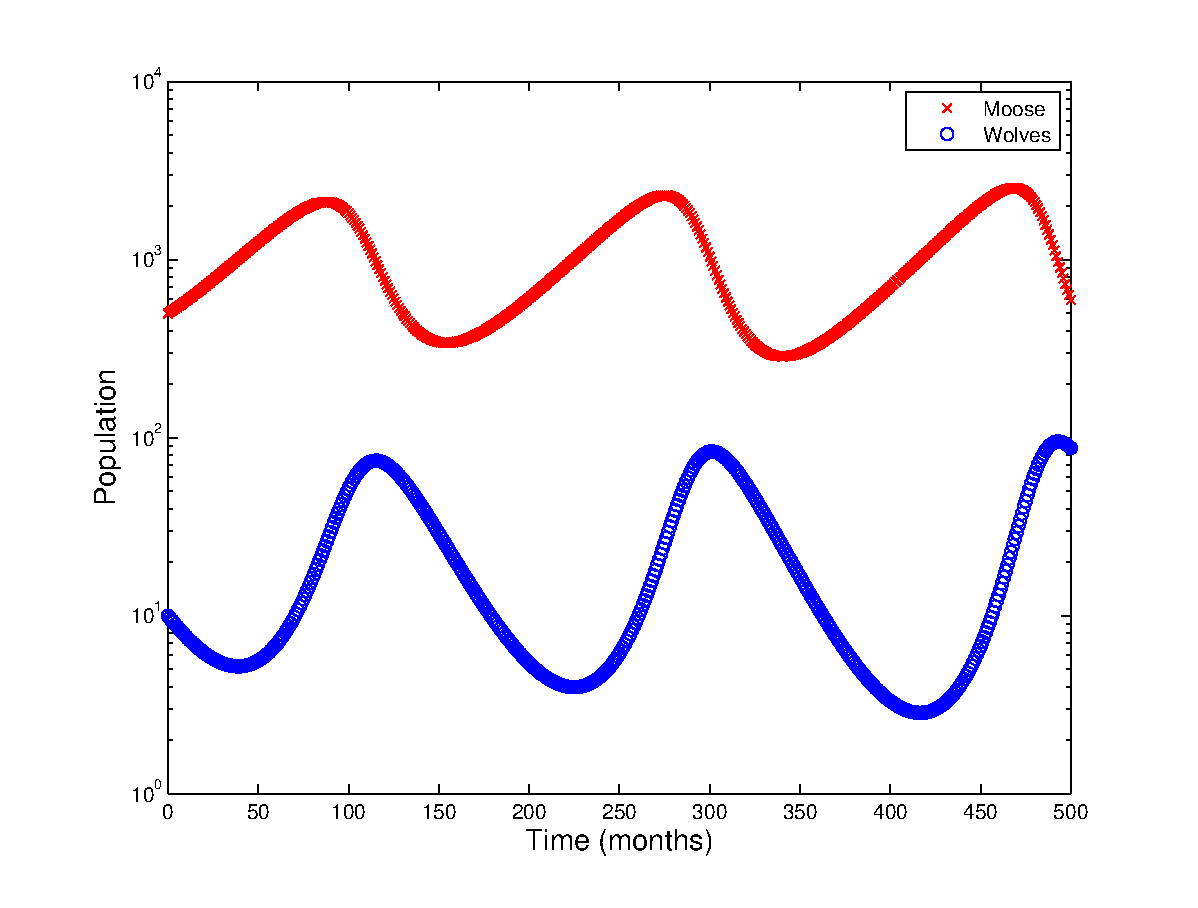
\includegraphics[width=4in]{figs/LogarithmicWolfMooseTimeSeries}
\caption{Comparison of timeseries results using a logarithmic y axis for Wolf-Moose System. Timestep of one month,   $\beta = 0.025, \gamma = 0.057, W_c = 25, M_c=1000, M(1) = 500, W(1) = 10$}
\end{figure}

\subsection{Don't leave yourself guessing}

A common shortcut in making plots is to just {\it make} the plot, but not to take the additional time to add axis labels, legends, captions, etc.  

You know what comes next:  {\it Resist this temptation.}  While it may be the case that, in the instant when you create the plot , you know precisely what the axes and colors mean, you will almost certainly return to the plot later in the day, week, or year, and wonder what the heck it was that you plotted, and how you generated the results.  

Furthermore, even when you are actively working with a plot, it's very easy to find yourself wondering whether the red or the blue symbols represented wolves.

So, even though it takes a little more time, you should always include axis labels; you should always label your data (e.g., with a legend); and you should always somehow record how the results were obtained (e.g., what the simulation parameters were).   

Yes, it takes extra time.  But it will save you a lot of time and potential embarrassment in the future.

\subsection{Rules of thumb for making plots while modeling}

We'll end this section with a couple of rules of thumb for facilitating comparison:
\begin{enumerate}
\item Never hesitate to make another plot.
\item Always get experimental data into digital form.
\item Data and results should be presented, as much as possible, using the same axes.
\item When two datasets or model outputs share either an x coordinate (e.g., time), or a y coordinate (e.g., moose population), they should share that axis as well.
\item It is almost never a good idea to produce a plot in which one of the datasets appears to be a flat line.
\item Always, always, always label your axes and your data series.  You should be able to return to the graph a month later and decipher it without significant pain.
\end{enumerate}

\clearpage

\section{Making plots for presentations}

Above we've discussed some of the guidelines for creating plots while you are working.  A related, but distinct, skill is the ability to make graphs that you will include in a poster or presentation.  There are a couple of aspects of this:  first, you need to {\it decide} what the plot is that you want to make; and second, you need to actually {\it execute} the plot in a professional manner.  We'll deal first with the decision-making, and then transition to the more nuts-and-bolts issues around creating professional-looking plots.


\subsection{What's the argument?}

When you are creating graphs as a part of the modeling process, you are often using them in order to decide what the story {\it is} -- i.e., you're using the graphs to enhance your understanding of the model or the physical situation.

On the other hand, when you are making plots or figures for a presentation, you are using them as evidence that you are presenting to an audience.  This evidence is in support of some argument that you are making.  You must be very intentional about what argument {\it you} want to make, while at the same time being aware of inconsistencies and weaknesses.  This then allows you to decide what graph, or collection of graphs, will be most effective in making that argument, {\it and} in highlighting the ways in which inconsistencies might undermine your argument.

\newthought{This is an awful lot like writing a paper:}  you need to explore the evidence, decide on your argument, and then you need to decide how you are going to present the evidence in a balanced way that supports the argument while not ignoring the evidence against your position.  Furthermore, the evidence you choose needs to be appropriate for your audience.

And, to the extent that it's like writing a paper, you need to spend some time thinking through your argument, creating drafts, and revising and refining your work until you have crafted a set of graphs (and other representations) that really make your point effectively for your assumed audience.  

\subsection{Confidence-builders, setups and punchlines}

A useful distinction in creating graphs and figures for presentation is to ask what {\it role} the graph plays in the presentation or the poster. 
 

\newthought{Confidence builders are graphs that say, ``Look, it works!''.}  In almost every setting you'll want to convince the audience that your model, and your simulation approach, are sensible.  To a certain extent you could label these as ``validation graphs'', in that they demonstrate that the model has the right kind of behavior, but there is a difference.  As a part of {\it your} modeling work, you should create validation graphs that allow you to convince {\it yourself} and your colleagues that your model is sensible.  On the other hand, when presenting your work, you need to decide what the right graph(s) are to show the audience that (or in what ways) your model ``works''.   Confidence -building graphs (and all graphs!) are also careful to {\it highlight inconsistencies} -- nothing undermines confidence like unacknowledged fishiness!

One example of a confidence-building graph you've already seen is the comparison of the simple wolf-moose model with the experimental data form Isle Royale (shown above, so we won't repeat it a third time).  By showing that the model can be made to match the data with at least qualitative fidelity, we are demonstrating to the audience that it can be, to a limited extent, trusted.  At the same time, acknowledging that the parameters used to achieve this fit are not the same as those that are experimentally observed is an important component of highlighting inconsistencies -- as is the observation that the actual drop in wolf populations was due to parvovirus. 

\newthought{A second variety of graph or figure is the ``setup graph''.}  This kind of figure typically used to explain what it is that you're examining.  Often such a graph will show the kinds of behavior that you are interested in, and might be used to define any {\it figures of merit} you are using.  As you may recall from the Isle Royale chapeter, figures of merit numbers that are extracted from a simulation, that characterize the behavior you're interested in.

Thinking back to the Isle Royale example, the plot that showed the behavior of the model for two different birthrates is an excellent example of a setup graph.  Below is a cleaned-up version of this plot (made more presentable for presentation purposes).

\begin{figure}[h!]
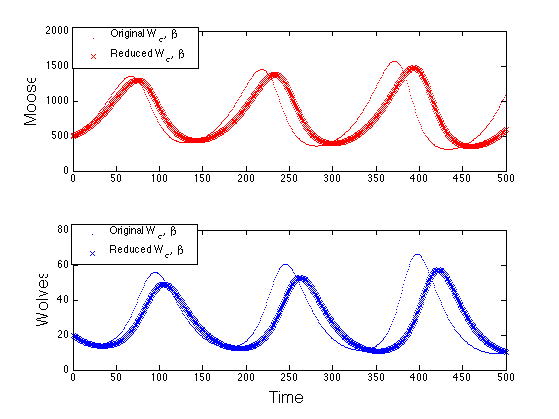
\includegraphics[width=4in]{figs/MooseBCTimeSeries}
\caption{Example of a setup graph for the Isle Royale caes.  Comparison of model results for different values of  $W_c$ and correspondingly changed 
$\beta$ shows the behavior of interest, and also provides a definition of the figures of merit (the initial period and amplitude).  Timestep of one month,  $\gamma = 0.05, M_c = 800, K=1$, original $W_c = 30$; reduced
$W_c = 27$.}
\end{figure}

On one hand, this graph shows the behavior that we're interested in:  the amplitude decreases, and the period increases, when the birthrate drops.  It shows this idea in a very credible way, using the kind of timeseries that we're used to seeing.  At the same time, it includes a graphical definition of the two figures of merit:  initial amplitude, and initial period.

\newthought{Punchline graphs bring the argument home for your audience.}  In the Isle Royale case, as we've noted, the definition of two figures of merit -- initial period and initial amplitude -- allow us to create plot that has a clear punchline:  `` for birthrates above .03, we expect the size of population oscillations to decrease and the period increases as we introduce birth control to the moose population.''  The figure makes this point directly -- but it only does so credibly if it is preceded by the setup graph, which shows how the system behaves and defines what is being plotted, and by the confidence-building graph, which makes the argument that the model can be trusted to behave something like the actual physical system.

Often punchline graphs are plots of figures of merit:  in the setup graph you define the figure of merit (e.g., the initial amplitude) and in the punchline graph you show that the figure of merit behaves in a particular way.  For the Isle Royale case, the punchline graph shows that the amplitude of moose oscillation decreases with decreasing moose birthrate, while the period increases.

\begin{figure}[h!]
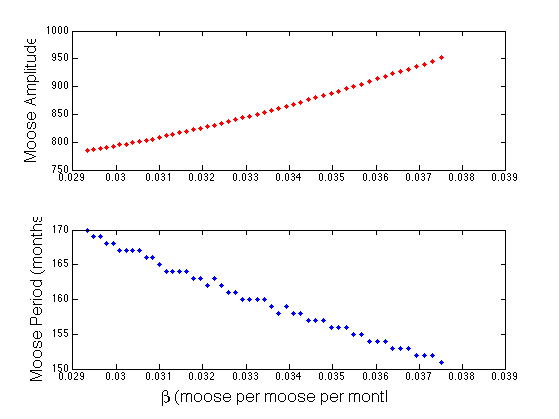
\includegraphics[width=4in]{figs/MooseBCSweepClean}
\caption{Example of a punchline graph for the Isle Royale case.  Amplitude and period of moose population for sweep of moose birth rate and critical wolf population $W_c$.  Timestep of one month,  $\gamma = 0.05, M_c = 800, K=1$.  Note that the period exhibits discrete steps due to the discrete time model.}
\end{figure}

\clearpage

\newthought{In short,} for this particular case, our argument boils down to something like the following:

\begin{enumerate} 
\item Our model works something like the real system:

\beforefig

\centerline{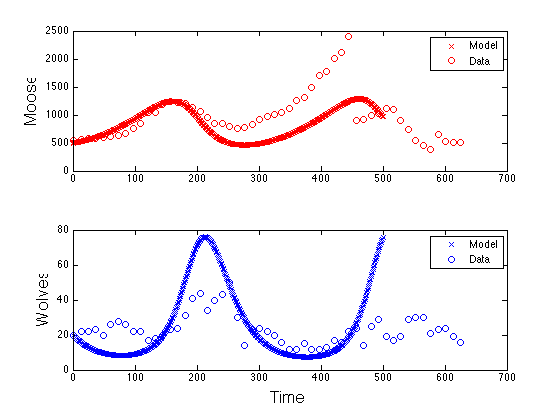
\includegraphics[width=2.5in]{figs/ModelDataComparison}} 


 
\item We observe that dropping the birthrate has an effect on the period and the amplitude of oscillations:

\beforefig

\centerline{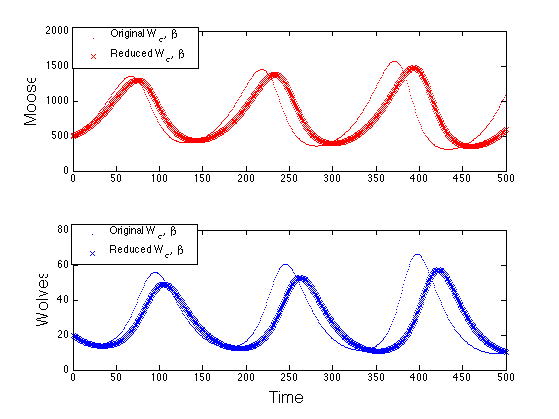
\includegraphics[width=2.5in]{figs/MooseBCTimeSeries}}

\item We find that, for a reasonably broad range of birthrates, the period increases and amplitude decreases as we reduce the birthrate:

\beforefig

\centerline{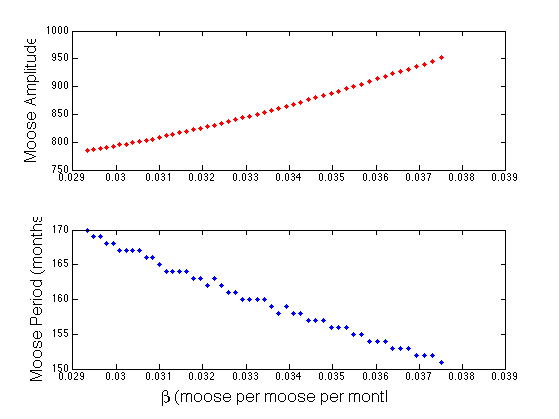
\includegraphics[width=2.5in]{figs/MooseBCSweepClean}}

  This suggests that in the real system, introduction of mild moose birth control might suppress the magnitude of population variability -- an interesting, and not altogether intuitive, result.


\end{enumerate}

\subsection{Make it clear, make it pretty}

So far we've been concerned with {\it what} to plot. If you compare the  plots in this chapter with many in the Isle Royale chapter, you'll note in the Isle Royale chapter we've been more than a little sloppy with the actual plots -- for example, the axis labels seem to be getting cut off; the fonts are rather pixellated; the choice of symbols is kind of amateurish -- these are really some rather unprofessional looking plots we've been using in most cases!

On the other hand we {\it hope} you've noted that some of the graphs in this chapter are actually quite pretty.  The fonts are legible; the axis labels are clear and complete; there is no gratuitous use of color or of extra ink.  

The reason for this difference is that, for this chapter, we've in general taken a bit of extra time to make the graphs clear and professional.  We could claim that our failure to do so in the Isle Royale chapter was intentional for pedagogical reasons, but then we'd be lying.  

In order to make a graph clear and professional, there are a couple of things you need to think about.  First, you should be aware of general guidelines for making good figures.  Edward Tufte provides a succinct set of these in his book, {\it The Visual Display of Quantitative Information}, which are somewhat adapted in the list below:
\begin{enumerate}
\item {\em Above all else, show the data}.  This implies that your emphasis in creating a plot should be on the data (including model predictions).  
\begin{enumerate}
\item Design plots that have a {\em high data-ink ratio}:  i.e., most of the ink used to create the plot is used to communicate information about the data.  
\item Design plots that {\em emphasize the data}.  Use heavier lines for data than for axes: the data should ``pop.''  Choose axis ranges that show the behavior of the data -- i.e., don't create a plot with enormous white space around a horizontal line, unless what you are showing is that the line is horizontal!  
\item Design plots that {\em assist the reader}.  Part of this has to do with facilitating comparison (as discussed above); and part of it has to do with minimizing the amount that the reader has to move his or her eye in order to get the information.  For example, legends are fine, but if you can directly label data in your plot, you avoid making the reader switch back and forth between the legend and the data, and you also reduce the amount of ink you use.
\item {\em Avoid ``chartjunk''}: It is often tempting to be cute in creating plots (think {\it USA Today}.  Unnecessary graphical elements (like 3D bars, background cartoons, drop shadows, obnoxious fonts, etc. hinder understanding. 
\end{enumerate}
\item {\em Tell the truth about the data.} You can create false impressions through your graphic design -- look back, for example, at figure 6, which graphically suggests a much better match than exists in reality.  Make sure you choice of axis scaling, axis alignment, etc. don't deceive the audience.
\item {\em Revise, revise, revise.}  The plot you first generate is almost never the plot you should present.  Take the time to make it better.
\end{enumerate}

The second thing you need to be aware of is the nuts-and-bolts of working with a figure -- i.e., going beyond the use of the {\tt plot} command.  You need to become familiar with the necessary tools and workflow for creating a good graph. In other words, the guidelines above are useful only if you can actually make them operational.


\newthought{So how should you edit a graph} to actually prepare it for inclusion in a poster or presentation?  In other words, how do you go from ugliness like MATLAB produces to prettiness like figure 13? We'll  assume that you already know what story you want the graph to tell, that you have made appropriate choices in portraying measurements versus model predictions, in deciding on nominal axis ranges, in labeling axes with units, etc. In other words, we're going to address the ``last 10\%'' of work on a graph. 

When you make a graph for a presentation, you typically put in a fair bit of additional care into the creation of the graph, from careful color choices and font sizing, to very intentional use of labeling, to removal of extraneous stuff that does not contribute to your point.

To do this well, it is often easiest to first generate the graph in MATLAB, and to do a bit of preliminary work in MATLAB, but then to finish cleaning up the graph in Illustrator, which gives you far more flexibility in putting on finishing touches.

Since we assume you are tired of wolves and moose, let's use as an example of a cat mortality graph.  Imagine, if you will, that I have a MATLAB code that produces a prediction of human and cat mortality as a function of number of stories the cat (or human) falls.  The model includes the cat's transition from regular position to ``flying squirrel position'', so that it helps to explain the anomalous drop in cat mortality for larger distances.

If we simply plotted the results in MATLAB and then used cut-and-paste to insert them in a document, we would get a very, very ugly figure.  If you're not sure about whether this approach gives you ugliness, just take a look at the figure below which highlights the the many ways in which this approach produces yuckiness...

\begin{figure*}[h!]
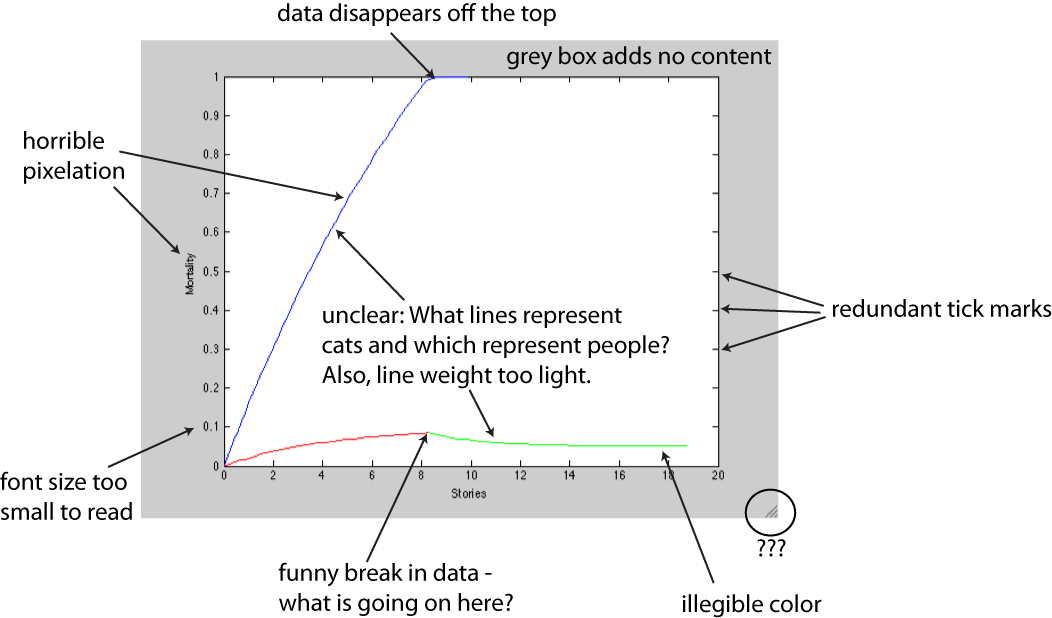
\includegraphics[width=6.5in]{figs/uglycatfigureannotated}
\caption{The result of cutting and pasting from MATLAB, annotated to highlight areas of horribleness.  See, I told you it was horrible.}
\label{fig:uglycatfigure}
\end{figure*}

Of course, we can partially rectify many of these faults within MATLAB. We can intentionally increase the weight of lines, add a legend, increase the fontsize, and at least being a bit more intentional about colors.

\begin{verbatim}
% Plot with a thicker line
plot(stories,humansurvival,'b', 'LineWidth',1.5) 

% Use a bigger font on axis labels and tick labels
xlabel('Stories','FontSize',14) 
set(gca,'FontSize',12)

% Turn off extra ticks, etc.
set(gca,'Box','off') 

% Set the axes so you can see the data
axis([0 17 0 1.1])

% Include a legend
legend('Humans','Cats') 
\end{verbatim}


We can also change the way we get the figure into our document -- rather than cutting and pasting, save it as a graphics file (e.g., a .png).  The result, shown below, is better, but not exactly inspiring (note: this is basically what we've been doing above).  The fonts are still illegible; the line widths and colors are still not great; the legend does the job, but does require a lot of work from the reader... And, the somewhat frustrating aspect of this is that you almost never know what, exactly, MATLAB is going to do when you export.   So creating figures that look consistent is a bit of a crapshoot at times.






\begin{figure}[h!]
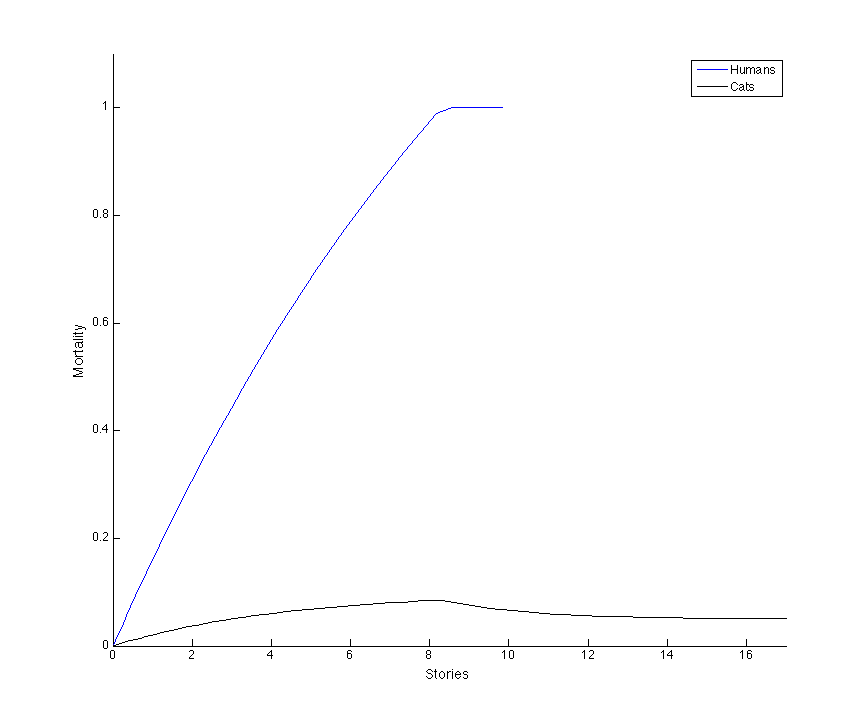
\includegraphics[width=4in]{figs/LessUglyCatFigure}
\caption{The result of saving from MATLAB as a .png.  Better, but not great.}
\end{figure} 



Given this, if we really want to make the figure presentable and consistent, the best option is to work first in MATLAB until it is almost done, and then to export it as an encapsulated postscript file, and then open it up in Illustrator to do final touch up, font fixes, etc.  Note that ``touch it up'' means ``make it easier to read/interepret'',  not ``change the data to support your contentions!''  Using this approach, it's pretty easy to edit the figure to a state that is acceptable, as shown below:

 \begin{figure}[h!]
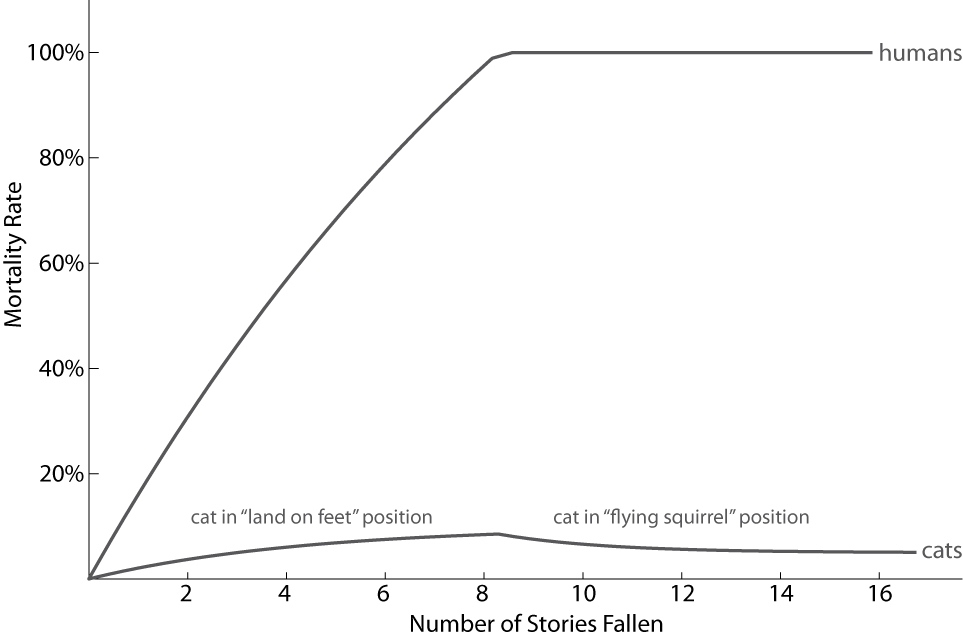
\includegraphics[width=4.25in]{figs/CatMortalityPrettified}
\caption{Prettified version of the cat mortality figure.}
\end{figure}
 
Now, this might not be perfect,  but it's pretty presentable.  There is no noticeable pixelation (and if I needed to, I could blow it up in Illustrator as much as necessary --- the only pixelation here is due to my exporting the .ai file for inclusion as a .png in this document.  There is very little extra ink: almost all the ink is serving a purpose for the audience.  The lines are directly labeled, so that the reader can immediately see what data is what --- no need to look to a legend.  The font sizes are nicely legible.  The lines ``pop'' relative to the axes, etc.  The reader can understand why the graph's features are present (i.e., the funny break is due to the cat's configuration changing as it falls).  And the labels are more self-explanatory:``Number of Stories Fallen'' tells a lot more than ``Stories''.

Here are some things to think about, and some advice for working with Illustrator and MATLAB. 
\begin{enumerate}
\item Be consistent.  Use consistent font and font size choices, consistent color choices, consistent labeling schemes, etc. 
\item Get rid of ink that doesn't do work.  In general, grids, boxes, grey borders, etc. are often not terribly useful.
\item Use heavier lines for data than for axes, etc.  The graph is there to show the data, so make the data ``pop''.
\item Associate labels directly with what you're plotting.  Although a legend does allow the reader to interpret the graph, it's better if the reader doesn't need to switch back and forth between a legend and the content.
\item Label salient features.  If there is a weird ``bump'' in a graph that will cause the reader to wonder what is going on, you should make clear what it is and why it's there.
\item Don't over-use color (just like you should not overuse ink).  In this graph, no color is necessary at all: there are two lines, and it is easy to distinguish which is which with a simple label.  Of course, if I had multiple graphs comparing cats and people, it might make sense to define a convention for cats versus people (e.g., cats = green lines, people = grey lines).  This would enhance the consistency (see above) from graph to graph.  
\end{enumerate}

When using MATLAB and Illustrator, 
\begin{enumerate}
\item Let MATLAB do as much work as you can.  Even though the second figure above is still some distance from presentation quality, the less editing you need to do in Illustrator, the better.  Using a standard set of format commands for your plots in MATLAB will help you to be consistent, and will reduce the amount of work you need to do in Illustrator.
\item Define your style features in Illustrator, and set them up, before you start playing too much.  By choosing your color swatches, line widths, fonts, etc. in advance, you can avoid the rathole that Illustrator can become.
\item MATLAB produces Illustrator files with a lot of extra boxes, out-of-date fonts, etc.  Save your figure as an .eps, and clean the file up before you start trying to fix the graphical issues. 
\end{enumerate}

\section{Further Reading}

This chapter only begins to scratch the surface of making plots and figures that support your work.  Edward Tufte's work is perhaps the best known guide to making good graphics; if you don't own copies of {\it The Visual Display of Quantitative Information} and {\it Visual Explanation}, you should go buy them.  Now.  Note: this is not an order.  It is a suggestion.  A very good suggestion, but a suggestion nonetheless.
